\documentclass[twocolumn,superscriptaddress]{revtex4-1}
\usepackage{amsmath}
\usepackage{graphicx}
\usepackage{xcolor}
\usepackage{braket}
\usepackage{tikz}
\usepackage{tikz-3dplot}
\begin{document}

\title{Assessing the importance of deep transition encoders for machine translation tasks}
\begin{abstract}
Machine translation is a challenging task and an active area of research in natural language processing.
A standard technique in use now for machine translation are sequence to sequence neural network composed of an encoder and decoder recurrent neural network architecture.
With the rise of fast and available GPU systems, deep architectures for machine translation have been proposed and shown to improve translation quality in a limited set of translation tasks \cite{DBLP:journals/corr/ChoMBB14, miceli-barone-etal-2017-deep}
In this study, I investigate whether the deep transition encoder proposed and studied in \cite{miceli-barone-etal-2017-deep}, yields benefit over a larger set of translation tasks.
I find that the benefits are consistently 1 $-$ 2 BLEU points across English to Italian, German, Portugese, French, and Spanish translation tasks, giving credence to the general benefit of deep encoders in machine translation. 
\end{abstract}
\maketitle

\section{Introduction}
Machine translation is a challenging task and an active area of research in natural language processing.
The task of machine translation is, given an input-output language pair, to translate text from the input language to the output.
The text in question can be single words, sentences, paragraphs, or entire books, with the intention of the translation being both adequate and fluent.
Here, adequacy indicates how well the translation can capture the meaning and intent original input sentence, and fluency measures how fluent the output language is.
While seemingly simple, the task of generating fluent and adequate translation is very challenging.

The standard for machine translation are sequence to sequence (seq2seq) neural network.
As the name suggests, these neural networks take a sequence of words as an input and translates it to sequence of output words in the target language.
This task is typically broken into two pieces: an encoding step where the input sequence is mapped to a fixed-length, encoded vector, and a decoder, where the encoded vector is decoded to a variable-length output sequence.
Simple seq2seq models with recurrent neural network (RNN) encoders and decoders have been shown to perform comparably to most statistical, non-neural models \cite{DBLP:journals/corr/ChoMBB14}, and the inclusion of basic modifications such as attention boost the seq2seq model accuracy far beyond what non-neural models can achieve \cite{bahdanau2016neural}.

More recently, there has been heavy focus in the field to modifications to the simple seq2seq model which can efficiently improve translation quality.
In particular, with the rise of fast and available GPU systems, deep architectures for machine translation have been a popular choice.
Deep transition decoder architectures like Nematus have been proposed and shown to improve translation quality significantly across a variety of translation tasks \cite{sennrich-etal-2017-university}.
An extension to this study looked at deep transition encoders as well, and other deep architectures \cite{miceli-barone-etal-2017-deep}.
They also found that the deep neural networks can increase BLEU score by 2 $-$ 4 points without increasing model complexity drastically.
Unfortunately, this study was limited to translation between English and German, leaving open the question of how well these novel deep models perform in other translation tasks.

In this report I investigate, in a quite limited way, the improvement in translation quality from using the novel models in \cite{miceli-barone-etal-2017-deep} when looking at various translation tasks.
I limit myself to just the deep transition encoder model with a shallow decoder with attention with a simpler training data set than used in the original study, but with translation between English and German, French, Italian, Portugese, and Spanish.
I found that across these translation tasks that the deep transition encoder improves the BLEU score by 1 $-$ 2, similar to  what was seen in the original paper.
While not conclusive, I believe my report gives some additional credence to the general benefit of the deep transition encoder of \cite{miceli-barone-etal-2017-deep} in machine translation.

\section{Data sets and processing}
Given the limited computer time and project time for this study, I opted to use a smaller, and simpler, data set for training and validation. 
The data sets for all the languages considered were taken from \url{http://www.manythings.org/anki/}.
This data set is simpler for two reasons.
First, the total corpus size is much smaller than the news translation task in \cite{miceli-barone-etal-2017-deep} with 100K $-$ 300K sentences in each corpus.
Second, the language in the translation task is much more formal and taken from news reports, whereas the bilingual sentence pairs here are basic sentences used for English as a second language audience.
The latter then has simpler sentence structures, leading to easier translation and less required model complexity to get reasonable translation quality.

The processing pipeline for the data is also quite simple.
Since all of the languages being used were in Latin script, the tokenization of words was done by spaces.
All punctuation was removed from sentences, all words were set to lowercase, and all embellishments (such as accents) on letters were removed.
Further, all sentence pairs had at most length 10 words, which allows for ease of translation.
Lastly, words which were used fewer than 100 times were replaced by the $\langle$ unk $\rangle$ token in all sentences.
After filtering, the corpus was split into 75$\%$ training data and 25$\%$ validation/testing data.

\section{Model architectures and training}

\begin{figure}
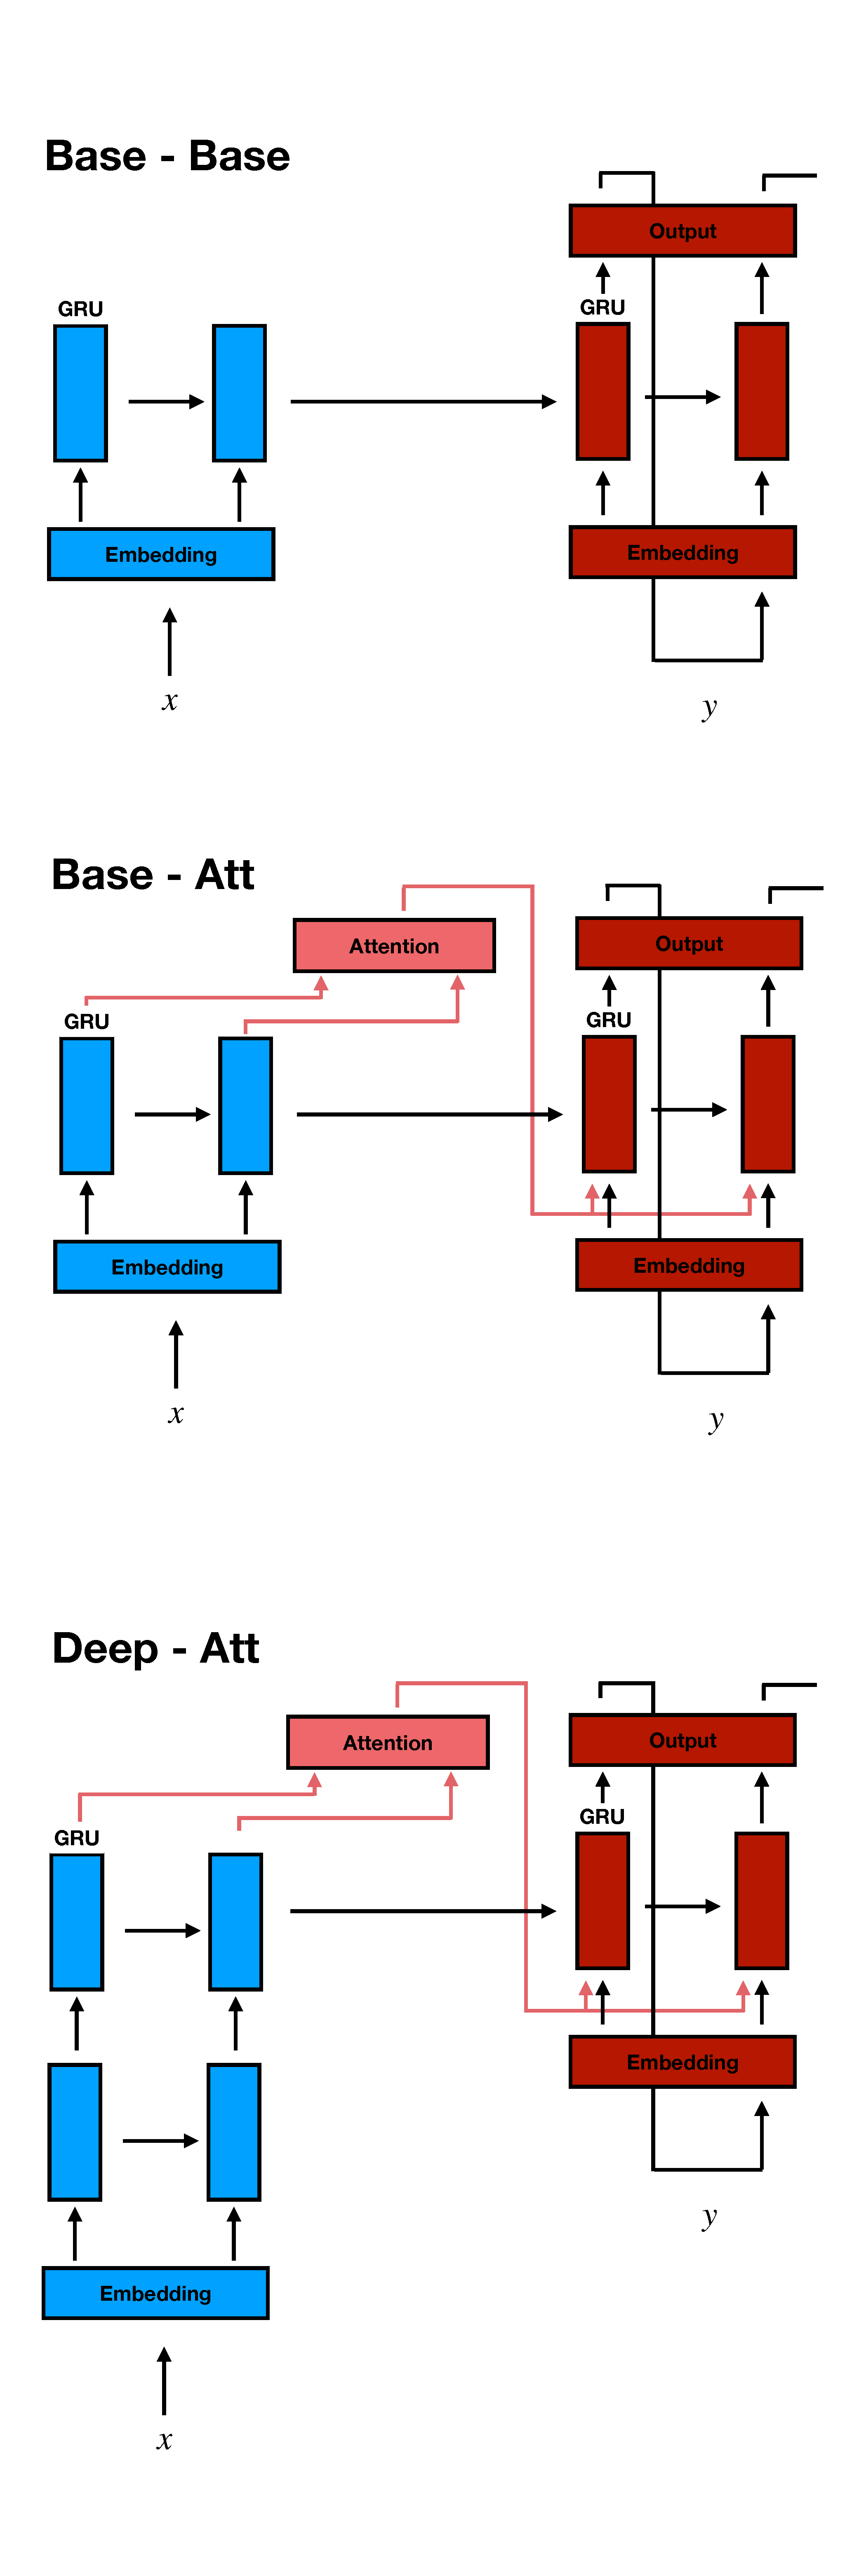
\includegraphics[scale = 0.15]{../plots/architecture.pdf}
\caption{
Three architectures used in this study from the simplest, Base-Base, at the top, to the most complex, Deep-Att, at the bottom.
The blue boxes refer to the encoder network, the red to the decoder, and pink the attention network.
The study focuses on the benefit from Base-Att to Deep-Att, which improvements from Base-Base to Base-Att as reference.
} 
\label{fig:architectures}
\end{figure}

For this study I used three model architectures, which can be seen in Figure ~\ref{fig:architectures}.
All three were simplified versions of the architectures seen in \cite{miceli-barone-etal-2017-deep}.
First is the base model, referred to as the Base-Base model, which is a seq2seq encoder-decoder model without any additional frills.
The encoder consists of an embedding layer which goes into a gated recurrent unit (GRU).
The hidden vector of this GRU gets forwarded into the initial hidden state of the decoder GRU, which also takes input through an independent embedding layer.
The output from the decoder GRU passes through a fully connected feed forward network that maps the hidden states to the output vocabulary.
The second network introduces the exact attention mechanism of Bahdanau \cite{bahdanau2016neural} into the decoder, and is referred to as the Base-Att network.
The third network introduces a deep transition decoder with a GRU network depth of 2.
The comparison between Deep-Att and Base-Att is what this study will be oriented around, the Base-Base to Base-Att improvements are for reference.

The technical specifications of the models are as follows: all network layers - embedding, GRU, attention, output, etc - all have size 128.
The first two models were trained from zeroed parameters for 200 epochs using a batch size of 10 000 sentences with the Adam optimizer and a learning rate of 0.001.
The last model was trained starting from zeroed parameters for the deep encoder and the optimized attention decoder parameters from the second model.
This choice was made to accelerate the training process and to avoid local minima in the optimization due to the heavy recurrence present in the deep encoder.
All calculations were done in PyTorch, with the code provided alongside this report.


\section{Results}
The results of the study are summarized in Table ~\ref{fig:table}. 
Presented are, for various translation tasks from English to the specified language the total number of model parameters, as well as four different BLEU scores. 
These four scores corresponding to different weightings in the BLEU metric for 1-, 2-, 3-, and 4-grams: BLEU1 has weight (1, 0, 0, 0), BLEU2 (0.5, 0.5, 0, 0), BLEU3 (0.33, 0.33, 0.33, 0), and BLEU4 (0.25, 0.25, 0.25, 0.25).

In order to study the results more concisely, a visualization of the BLEU4 score improvement with model complexity is presented in Figure ~\ref{fig:barplot}.
Here we see three interesting facts.
First, the improvement due to attention is extremely large, typically of order 10 points, whereas the additional improvement from the deep encoder is of order 1 point.
This indicates that the attention mechanism is extremely important in acquiring higher BLEU score, and presumably higher translation quality.
The deep encoder serves as a secondary mechanism, and while small, is not an insignificant change, in particular for the Italian task, which in this case increased by 2.1.
Second, the improvement from the deep encoder is very consistent across the five different translation tasks.
This indicates that the deep architecture is able to generally capture features of required for translation, not just features which are specific to the structure of a particular language.
Thirdly, the returns seem to be diminishing, namely that roughly 100K new parameters are introduced at each level of complexity, but the deep encoder returns only 1/10 the benefit of the attention mechanism.
This is a standard pattern we see in most model development and should not be too concerning, but having a rough estimate of the diminishing return, in this case 1/10, is a useful rule of thumb.

This study is of course limited, for a variety of reasons.
First, the corpus being trained on does not include complex sentences, and thus serves as a very shallow representation of most languages.
Second, the architectures I used were correspondingly simpler, and as such my results may over represent the benefits of the deep encoder.
Indeed, in \cite{miceli-barone-etal-2017-deep}, the largest improvement from the deep encoder, using a transition depth of 4, was just over 0.5 BLEU, about 4 times smaller than what I observe.
Lastly, the languages I selected are not representative of the large linguistic variation that exists in written languages.
As such, to get more conclusive statements of the benefits of these deep architectures, much more extensive work is required.

\begin{table}
French \\ 
\begin{tabular}{lrrrrr}
\toprule
          Model &  Params &   BLEU1 &   BLEU2 &   BLEU3 &   BLEU4 \\
\midrule
           Base &  560455 &  58.261 &  40.780 &  29.350 &  23.052 \\
      Attention &  626376 &  67.889 &  53.907 &  42.483 &  34.856 \\
 Deep Attention &  725448 &  69.058 &  55.411 &  44.059 &  36.338 \\
\bottomrule
\end{tabular}
 \\ 
German \\ 
\begin{tabular}{lrrrrr}
\toprule
          Model &  Params &   BLEU1 &   BLEU2 &   BLEU3 &   BLEU4 \\
\midrule
           Base &  635019 &  61.709 &  42.844 &  30.862 &  24.540 \\
      Attention &  700940 &  68.164 &  51.383 &  39.427 &  32.279 \\
 Deep Attention &  800012 &  69.502 &  53.033 &  41.214 &  34.009 \\
\bottomrule
\end{tabular}
 \\ 
Italian \\ 
\begin{tabular}{lrrrrr}
\toprule
          Model &  Params &   BLEU1 &   BLEU2 &   BLEU3 &   BLEU4 \\
\midrule
           Base &  765210 &  62.758 &  46.850 &  36.379 &  29.542 \\
      Attention &  831131 &  72.786 &  60.997 &  51.073 &  43.221 \\
 Deep Attention &  930203 &  74.061 &  62.757 &  53.096 &  45.296 \\
\bottomrule
\end{tabular}
 \\ 
Portugese \\ 
\begin{tabular}{lrrrrr}
\toprule
          Model &  Params &   BLEU1 &   BLEU2 &   BLEU3 &   BLEU4 \\
\midrule
           Base &  539781 &  64.503 &  48.221 &  36.353 &  29.310 \\
      Attention &  605702 &  73.920 &  61.357 &  50.156 &  42.165 \\
 Deep Attention &  704774 &  74.541 &  62.273 &  51.303 &  43.417 \\
\bottomrule
\end{tabular}
 \\ 
Spanish \\ 
\begin{tabular}{lrrrrr}
\toprule
          Model &  Params &   BLEU1 &   BLEU2 &   BLEU3 &   BLEU4 \\
\midrule
           Base &  478672 &  65.336 &  48.556 &  35.846 &  28.290 \\
      Attention &  544593 &  71.209 &  57.435 &  45.270 &  36.956 \\
 Deep Attention &  643665 &  72.299 &  58.727 &  46.777 &  38.362 \\
\bottomrule
\end{tabular}
 \\ 

\caption{
Results from the different models fit in this study.
Presented are the different tasks, models, the number of parameters, and the four BLEU scores that were computed.
}
\label{fig:table}
\end{table}

\begin{figure}
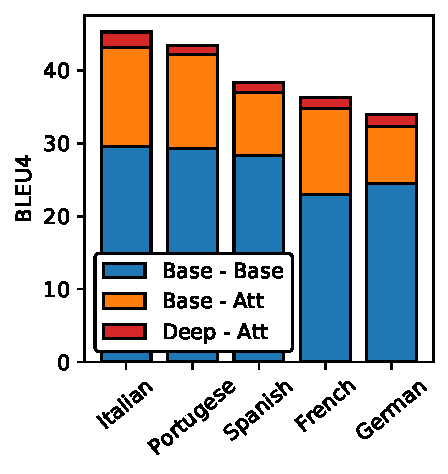
\includegraphics{../plots/barplot.pdf}
\caption{
Summary of the BLEU4 score improvements found in this study across the different translation tasks, English to various languages.
The heights of the colored bars refer to the improvement with each addition to the network.
}
\label{fig:barplot}
\end{figure}

\section{Conclusion}
In this study I attempted to generalize the results of \cite{miceli-barone-etal-2017-deep} to various translation tasks, in order to determine the importance of deep architectures in neural machine translation.
I found that, that the deep encoder helps improve BLEU score by 1 - 2 for the English to German task.
I further found that the improvement is similarly 1 - 2 BLEU points across 5 tasks, English to Italian, Portugese, Spanish, French, and German.
Lastly, I found that the benefits of the deep encoder are about 1/10 that of attention in improving BLEU.
This indicates that while the deep encoder yields a significant improvement to translation quality, the work-horse of the model lies with a good attention model.
My results give credence to the idea that deep encoders can help improve neural network translation quality, and gives a nice rule of thumb: the attention network does 10 times as much work as the deep architectures.

\bibliography{Manuscript.bib}

\end{document}